\section{Tickets aggregation}
The word aggregation means the process of combining things or amounts into a single group. 
HOPR adds an additional scaling layer that aggregates multiple tickets and redeems them within one transaction.
\\~\\ Since probabilistic payments cannot scale arbitrarily and ethereum gas fees are only increasing it makes sense to aggregate multiple tickets and redeem them within one transaction.
The preimage of a winning tickets stored in the node’s database. 
\\~\\ The node sends ticket or several winning tickets $ticket_A$ and $ticket_B$ with the corresponding pre-images to the issuer who computes their aggregation $ticket_C$. 
\\~\\The issuer stores on chain $h(ticket)$ of the redeemed tickets in a space-efficient data storage called Bloom Filters.
The issuer computes the modified Bloom Filter by XORing the previous version with the one after inserting the ticket.
\newline Once $ticket_C$ is sent to the smart contract, the intended version of the modified Bloom Filters is recovered by $bloom_{n+1} = bloom_n \vee diff$ and thereby invalidates $ticket_A$, $ticket_B$ as well as $ticket_C$.

\begin{figure}[H]
    \centering
    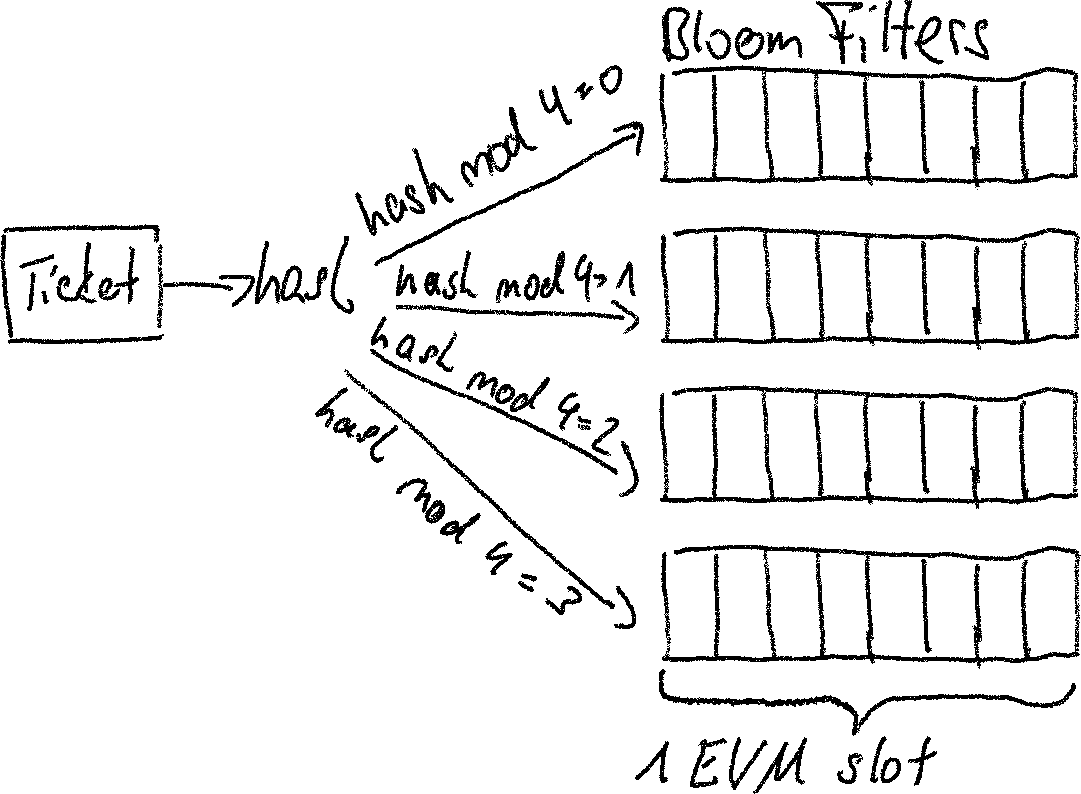
\includegraphics[width=10cm,height=10cm,keepaspectratio]{../yellowpaper/images/ticket_aggregation.png}
    \caption{Ticket aggregation}
    \label{fig:Ticket aggregation}
    \end{figure}
